% !TEX encoding = UTF-8 Unicode
% !TEX TS-program = xelatex

\documentclass[11pt]{article}

\usepackage{xspace}
\usepackage{fontspec,xltxtra,xunicode}
\defaultfontfeatures{Mapping=tex-text}
\setromanfont{Hoefler Text}
\setsansfont[Scale=0.94]{Gill Sans}
\setmonofont[Scale=0.9]{Lucida Sans Typewriter}

\newcommand*{\apple}{Apple\textsuperscript{\textregistered}\xspace}
\newcommand{\uti}[1]{{\ttfamily{#1}}}

\usepackage{microtype}
\usepackage{graphicx}
\usepackage[margin=1in]{geometry}
\usepackage{multirow}

\usepackage{fancyhdr}
\pagestyle{fancy}
\rhead{\today}
\chead{}
\lhead{\textbf{Uniform Type Identifers for Mac\TeX}}
\lfoot{Adam R. Maxwell}
\cfoot{}
\rfoot{\thepage}

\usepackage{color}
\usepackage{listings}
\usepackage{pdflscape}

% thanks to http://tex.stackexchange.com/questions/10255/xml-syntax-highlighting
\definecolor{gray}{rgb}{0.4,0.4,0.4}
\definecolor{darkblue}{rgb}{0.0,0.0,0.6}
\definecolor{cyan}{rgb}{0.0,0.6,0.6}
\lstdefinelanguage{plist}
{
  morestring=[b]",
  morestring=[s]{>}{<},
  morecomment=[s]{<?}{?>},
  stringstyle=\color{black},
  identifierstyle=\color{darkblue},
  keywordstyle=\color{cyan},
  basicstyle=\small\ttfamily,
  showstringspaces=false,
  morekeywords={xmlns,version,type}
}

\usepackage{hyperref}

\begin{document}

% because I'm too lazy to break the UTIs plist keys manually
\sloppy

% default to coloring comments green
\lstset{commentstyle=\color[rgb]{0.02, 0.62, 0.14}}

\section{Introduction}    
The present document intends to provide a brief overview
of the \apple Uniform Type Identifier (UTI) system and recommendations
for usage with \TeX{} document types. It is mainly intended as a reference for
developers who will be writing \TeX -related software on Mac OS X.

\subsection{What is a UTI?}
A UTI is a string which represents an abstract “type,” or class of entities, to
use \apple terminology,%
\footnote{\url{http://developer.apple.com/library/mac/\#DOCUMENTATION/FileManagement/Conceptual/understanding_utis/understand_utis_conc/understand_utis_conc.html}}
and file entities will be the focus of this discussion (\textit{e.g.}, \TeX{} files
that sit on your hard drive).
The UTI describes the file type uniquely, and is merely a way
of tagging it so that the system and other software can understand how to handle it.
For example, a plain text file is identified as \uti{public.plain-text}, which
is a UTI that is defined by \apple in the operating system. Only \apple is allowed
to create UTIs in the \uti{public} domain. In general, the owner is advised to use
a reverse-DNS prefix, such as \uti{com.adobe} as in the \uti{com.adobe.pdf} UTI
assigned to the PDF type.

\subsubsection{Inheritance}
One of the distinguishing concepts of the UTI type system is inheritance,
whereby a file is declared to descend from a root type. For the simple
cases, this is relatively obvious; for instance, it seems clear that
\uti{public.plain-text} would descend from \uti{public.text}. However,
UTIs also support multiple inheritance, so a file can descend
from otherwise unrelated content types. For example,
OmniGraffle\footnote{\url{http://www.omnigroup.com/products/omnigraffle/}}
files have a tree as shown in Figure~\ref{fig:graffle}.
\begin{figure}[htbp]
    \centering
        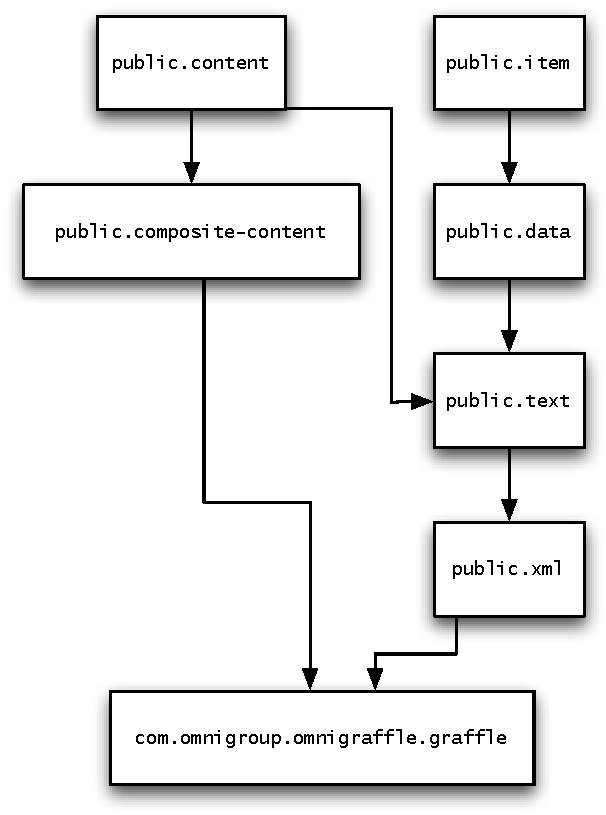
\includegraphics[height=3in]{graffle}
    \caption{OmniGraffle UTI inheritance tree}
    \label{fig:graffle}
\end{figure}
Notice how \uti{public.text} descends from \uti{public.data} and
\uti{public.content}; in essence, the former indicates its representation
in the system (a byte stream), and the latter its function (user-viewable content).
This also means that an application which can open any one of these
types can open an OmniGraffle file, so you can open it in your favorite
text editor or XML editor, and view some representation of the data.

\subsection{How are they used?}
The main use of a UTI that we are concerned with is to allow applications
to declare which file type(s) they can open. For instance, an application could
claim to open any \uti{public.image} file, or it could only claim to handle
\uti{public.jpeg} if its functionality was more limited. For proprietary
file types (\textit{viz.}, those not declared by \apple), developers must
include a definition of the file type and its identifying characteristics.

In addition, the UTI is used to determine which Spotlight importer to use
to search the content of a file, and it is used by Quick Look to determine
which plugin to use for previewing that file or creating icons. Likewise,
Finder uses the type to assign an icon to the file, if you are not using
Quick Look to create icons dynamically.

\subsubsection{Association}
A common misconception is that a UTI can be assigned to a specific 
file or file type. This is not the case. Rather, Mac OS X infers the UTI of a file
using metadata associated with that file, such as its name or the HFS type/creator
code embedded in the file. 
For data transmitted over a network, the MIME type may also be used
(though it's not clear if \apple actually uses it at this time).

Although a UTI is not the same as a file extension such as the “.pdf” typically
found on the end of an Adobe\textsuperscript{\textregistered} PDF file name,
current versions of Mac OS X consider the extension as the primary
form of metadata, overriding HFS type and creator code information if
present.\footnote{\url{http://tidbits.com/article/10537}} This causes
some confusion among users and developers alike, and is possibly the weakest 
point in Mac OS X's usage of UTIs, as there is now no way to resolve 
conflicts between files that have the same extension
but contain different data types. For instance, a “.img” file may
be a disk image, or it may be a raster image file, but when you double-click on
that file to open it in Finder, the system will attempt to open it in the default
application for that UTI. Since the UTI is based on the file's extension,
it may well open in the wrong application! You can usually work around this
by opening a file from within a given application, but this is not possible for
Spotlight and Quick Look plugins.%
\footnote{\url{http://lists.apple.com/archives/quicklook-dev/2008/Feb/msg00005.html}}%
\textsuperscript{,}%
\footnote{\url{http://lists.apple.com/archives/quicklook-dev/2008/Feb/msg00006.html}}

\subsubsection{Declaration}
A UTI is typically declared in the Info.plist file of an application
bundle on Mac OS X, as in this fragment from \apple documentation:%
\footnote{\url{http://developer.apple.com/library/mac/\#DOCUMENTATION/FileManagement/Conceptual/understanding_utis/understand_utis_declare/understand_utis_declare.html}} 
\lstset{language=plist}
\begin{lstlisting}
<key>UTExportedTypeDeclarations</key>
       <array>
           <dict>
               <key>UTTypeIdentifier</key>
               <string>public.jpeg</string>
               <key>UTTypeReferenceURL</key>
               <string>http://www.w3.org/Graphics/JPEG/</string>
               <key>UTTypeDescription</key>
               <string>JPEG image</string>
               <key>UTTypeIconFile</key>
               <string>public.jpeg.icns</string>
               <key>UTTypeConformsTo</key>
               <array>
                   <string>public.image</string>
                   <string>public.data</string>
               </array>
               <key>UTTypeTagSpecification</key>
               <dict>
                   <key>com.apple.ostype</key>
                   <string>JPEG</string>
                   <key>public.filename-extension</key>
                   <array>
                       <string>jpeg</string>
                       <string>jpg</string>
                   </array>
                   <key>public.mime-type</key>
                   <string>image/jpeg</string>
               </dict>
           </dict>
       </array>
\end{lstlisting}
There are at least two important points to make here.
\begin{enumerate}
    \item
    The definition includes a significant amount of ancillary data, such as
    a URL pointing to the reference documentation.
    \item
    Multiple tags are defined, including an HFS type code ('JPEG'), two
    extensions (“.jpeg” and “.jpg”), and the MIME type (“image/jpeg”).
\end{enumerate}
You can define a UTI with less information, but it's best to include
as much as possible, since it serves as a reference for users or developers.

Actually using the UTI is another matter, and depends on the type of bundle
(standalone application, Quick Look plugin, Spotlight plugin) you are developing.
Refer to the appropriate \apple documentation for details, though it's something
of a mess, due to rampant duplication of information. The Info.plist documentation%
\footnote{\url{http://developer.apple.com/library/mac/\#documentation/General/Reference/InfoPlistKeyReference/Introduction/Introduction.html}} is a reasonable starting point. \emph{Be very careful if you
mix UTI and classic type declarations in an NSDocument-based application!}
Support for UTIs varies across operating system versions, and some rather
bizarre problems can occur.\footnote{\url{http://www.omnigroup.com/mailman/archive/macosx-dev/2007-November/060638.html}}

\subsubsection{Conflicts}\label{sec:conflicts}
The preceding example uses the \texttt{UTExportedTypeDeclarations} key to declare
the UTI. A \texttt{UTImportedTypeDeclarations} key is also available, and is
recommended when you are declaring a type that you do not own, or when the
owning application may not be present on the system. For instance, if you
wrote an application that could read OmniGraffle files, you would declare
the \uti{com.omnigroup.omnigraffle.graffle} UTI in a 
\texttt{UTImportedTypeDeclarations} section of your application's Info.plist
file. This would allow the system to associate your application with OmniGraffle
files when OmniGraffle itself is not installed, but would not override
Omni's \texttt{UTExportedTypeDeclarations} when OmniGraffle is installed.

There are some additional subtleties not covered in the official
documentation. For example, if two applications declare a different UTI for the
same tag, both using \texttt{UTImportedTypeDeclarations},
this can lead to non-deterministic behavior and failure to open
files.\footnote{\url{http://www.omnigroup.com/mailman/archive/macosx-dev/2009-May/062244.html}}
Such conflicts are exceedingly painful to debug, particularly for users
who have no idea why their file icons are randomly changing, or the wrong
application is being used to open their files.

\subsubsection{Debugging}
There are several useful tools for debugging problems with file types and
UTIs. The first is \textbf{mdls(1)}, which can be used from the command
line to determine which UTI is associated with a given file. For example,
here is the output for the OmniGraffle file used to create Figure~\ref{fig:graffle}:
\begin{verbatim}
    $ mdls UTIDiagram.graffle 
    kMDItemContentCreationDate     = 2011-10-29 00:12:42 +0000
    kMDItemContentModificationDate = 2011-10-29 00:17:37 +0000
    kMDItemContentType             = "com.omnigroup.omnigraffle.graffle"
    kMDItemContentTypeTree         = (
        "com.omnigroup.omnigraffle.graffle",
        "public.composite-content",
        "public.content",
        "public.xml",
        "public.text",
        "public.data",
        "public.item"
    )
    kMDItemDateAdded               = 2011-10-29 00:17:37 +0000
    kMDItemDisplayName             = "UTIDiagram.graffle"
    kMDItemFSContentChangeDate     = 2011-10-29 00:17:37 +0000
    kMDItemFSCreationDate          = 2011-10-29 00:12:42 +0000
    kMDItemFSCreatorCode           = ""
    kMDItemFSFinderFlags           = 1024
    kMDItemFSHasCustomIcon         = 1
    kMDItemFSInvisible             = 0
    kMDItemFSIsExtensionHidden     = 0
    kMDItemFSIsStationery          = 0
    kMDItemFSLabel                 = 0
    kMDItemFSName                  = "UTIDiagram.graffle"
    kMDItemFSNodeCount             = 132986
    kMDItemFSOwnerGroupID          = 80
    kMDItemFSOwnerUserID           = 501
    kMDItemFSSize                  = 132986
    kMDItemFSTypeCode              = ""
    kMDItemKind                    = "OmniGraffle document"
    kMDItemLastUsedDate            = 2011-10-29 00:12:43 +0000
    kMDItemLogicalSize             = 132986
    kMDItemPhysicalSize            = 135168
    kMDItemUseCount                = 2
    kMDItemUsedDates               = (
        "2011-10-28 07:00:00 +0000"
    )
\end{verbatim}
The most relevant parts for our discussion are \texttt{kMDItemContentTypeTree},
\texttt{kMDItemContentType}, and \texttt{kMDItemKind}. These correspond to
\texttt{UTTypeConformsTo}, \texttt{UTTypeIdentifier}, and \texttt{UTTypeDescription},
respectively. You still may wonder where these come from, though, and
\textbf{mdls(1)} doesn't help with that! 

For further debugging, you need to use the \textbf{lsregister} tool, located at
/System/Library/Frameworks/\discretionary{}{}{}%
CoreServices.framework/Frameworks/\discretionary{}{}{}%
LaunchServices.framework/Support/lsregister 
(in Mac OS X 10.7; may be different in previous systems). Note that you
must use the full path, as this command is not available in the shell's
default search path.
Use the \texttt{-help} option to see a summary of
usage, but the most useful option is \texttt{-dump}, which dumps the contents
of the registration database to standard output as plain text. For the
OmniGraffle document, we find the following:
\begin{verbatim}
	type	id:            29764
		uti:           com.omnigroup.omnigraffle.graffle
		description:   OmniGraffle document
		flags:         exported  active  trusted  
		icon:          
		conforms to:   public.composite-content, public.xml
		tags:          .graffle
\end{verbatim}
From this, we discover that it is an “exported” UTI, that it has
multiple conformance, and a single tag. The same information
could be found by examining OmniGraffle's Info.plist at
\texttt{OmniGraffle.app/Contents/Info.plist}, but this is very useful
if you are trying to figure out which applications are claiming a type
or tag.

For debugging Quick Look plugins and Spotlight importers, use
\textbf{qlmanage(1)} and \textbf{mdimport(1)}, respectively. Note that
their debug options are very useful, as they can tell you exactly which
plugin is being used. Launch Services will commonly end up using an
old plugin, even one that is in the trash, if you are actively developing.
This can lead to much frustration with the system.

\section{\TeX{} and UTI}
We have probably spent an excessive amount of time introducing UTIs, when
a simple link to the relevant \apple documentation would suffice. However,
the official documentation does not discuss conflicting UTI definitions or
some of the other issues raised here. In this section, we discuss the
motivation for writing this document, and our hope that developers will
agree to adopt common set of UTIs for \TeX{} and its ancillary documents.
At present, we have competing definitions, largely because no standard 
exists, and there is no central clearinghouse for non-proprietary UTI 
definitions.

\subsection{Prefix}
In the case of \TeX{} and ancillary files, a “public” UTI seems appropriate,
since it has been available to the public for many years. However, 
the \href{file://localhost/System/Library/Frameworks/CoreServices.framework/Versions/A/Frameworks/LaunchServices.framework/Versions/A/Headers/UTType.h}{UTType.h} 
header\footnote{To quickly open this header file in Terminal, you can use
\texttt{open -h UTType.h}.  Likewise, you can use \texttt{open -h UTCoreTypes.h} 
to see the system definitions of various UTIs and their named constants.}
on Mac OS X contains the following comment:
\lstset{language=C}
\begin{lstlisting}
/*
  Types which are standard or not controlled by any one organization 
  are declared in the "public" domain. Currently, public types may  
  be declared only by Apple.
*/
\end{lstlisting}
This requires us to declare a non-public UTI for a public type, since
we are not \apple, and only \apple can mandate a UTI for a type that it
does not own. We understand the reasoning behind \apple reserving the
public domain for their own use on Mac OS X, but find it ironic nonetheless.

We propose the prefix of \uti{org.tug.tex} for \TeX{} and related file
types on Mac OS X. Alternatives include \uti{edu.stanford.knuth} or
\uti{comp.text.tex}. We do not have any claim over either of these, and
more importantly, we cannot establish a \texttt{UTTypeReferenceURL} at
either of them. A better alternative is \uti{public-texmf}, which is
a clearly neutral option, and would be acceptable with any domain.
This would require changing the UTI definitions of all shipping applications
that we are aware of\footnote{BibDesk and TeX Live Utility use \uti{org.tug.tex}}, 
but that is a one-time inconvenience to developers and users
(assuming that users update to the latest version).

\subsection{Suffixes}
The set of suffixes is determined by the number of file types used and
generated by \TeX{} and associated programs such as Bib\TeX; in general,
these will be filename extensions.
When this topic was discussed on the Mac\TeX{} Technical Working Group
mailing list, a large list of extensions was developed,
and it was soon evident that it would not be reasonable to declare all
of them as TeX file types. A non-exhaustive list is presented here for
illustration:
.tex, .ltx, .ctx, .bib, .bst, .aux, .dvi, .xdv, .sty, .cls, .bbl, .blg,
.brf, .fmt, .idx, .ilg, .ind, .ini, .mp, .toc, .log, .out, .synctex, 
.mem, .tfm, .vf, .pl, .vpl, .enc, .map, .lig, 
.tui, .tuo, .tub, .mps, .mpo, .mpy, .mpx, .rlg, .rlx.
Of these, not all are guaranteed to represent a \TeX -related file;
.ini and .log being two notable examples.

We propose that suffixes be added only as required, in order to avoid
conflicting UTIs (see Section~\ref{sec:conflicts}). In this context,
“required” means that your application requires that file for its
functionality, or provides some unique capability (such as syntax
highlighting). 
Further, we suggest that obviously ambiguous tags such as .ini and .log
never be associated with \TeX -related UTIs.

\section{Proposed Base Types}
Table~\ref{tab:proposedtypes} describes our proposed set of types that
would be suitable for most applications that handle \TeX -related files
on Mac OS X. We consider these types to be unambiguously related to \TeX, 
and they are required by one or more currently shipping applications on
Mac OS X.
\begin{landscape}
\begin{table}
\begin{tabular}{lllllll}
& \textbf{UTTypeIdentifier}& \textbf{UTTypeDescription} & \textbf{UTTypeConformsTo} & \textbf{Extension} & \textbf{MIME Type} & \textbf{HFS} \\
\noalign{\smallskip}
\hline
\noalign{\smallskip}
\multirow{7}{*}{\rotatebox{90}{\textbf{Input}}}
& \uti{org.tug.tex}              & TeX Document      & \uti{public.plain-text} & .tex  & application/x-tex   & TEXT \\
& \uti{org.tug.tex.context}      & ConTeXt Document  & \uti{org.tug.tex}       & .ctx  & text/plain          & TEXT \\
& \uti{org.tug.tex.latex}        & LaTeX Document    & \uti{org.tug.tex}       & .ltx  & application/x-latex & TEXT \\
& \uti{org.tug.tex.latex.style}  & LaTeX Style       & \uti{org.tug.tex.latex} & .sty  & text/plain          & TEXT \\
& \uti{org.tug.tex.latex.class}  & LaTeX Class       & \uti{org.tug.tex.latex} & .cls  & text/plain          & TEXT \\
& \uti{org.tug.tex.bibtex}       & BibTeX Database   & \uti{public.plain-text} & .bib  & text/plain          & TEXT \\
& \uti{org.tug.tex.bibtex.style} & BibTeX Style      & \uti{public.plain-text} & .bst  & text/plain          & TEXT \\
\noalign{\smallskip}
\hline
\noalign{\smallskip}
\multirow{7}{*}{\rotatebox{90}{\textbf{Output}}}
& \uti{org.tug.tex.dvi}          & DVI Document      & \uti{public.data}       & .dvi  & application/x-dvi   & \multirow{4}{0.5in}{DDVI\\ ODVI\\ $*$DVI\\ DVI2} \\
\\
\\
\\
& \uti{org.tug.tex.xdv}          & XDV Document      & \uti{public.data}       & .xdv  & application/octet-stream & \\
& \uti{org.tug.tex.aux}          & LaTeX Auxiliary   & \uti{public.plain-text} & .aux  & text/plain          & TEXT \\
\end{tabular}
\caption{Proposed type definitions for typical applications, separated by usage.
“Extension” refers to \texttt{public.filename-extension}, 
“MIME Type” refers to \texttt{public.mime-type}, and
“HFS” refers to the \texttt{com.apple.ostype} key.}
\label{tab:proposedtypes}
\end{table}
\end{landscape}
Note that .tex is commonly used as an extension for multiple file types,
so there is no guarantee that a .tex file is not \LaTeX, rather than plain \TeX.
Since Launch Services considers the extension to be the primary metadata in
this case, the opening application or bundle will have to determine the
actual type by sniffing the content. This may present some difficulty in
mapping internal types used by NSDocument to your UTIs.

\subsection{Adding to the list}
When adding a new UTI, first consider that the primary usage is by
Launch Services. The UTI is used to determine which application(s)
can open a given file, which Spotlight importer should be used for
that file, and which Quick Look plugin should be used to preview it. 
If you need one or more of those, then you should add a new UTI.
We recommend that you use \uti{public.plain-text} for plain text files,
and \uti{public.data} for any binary data files. For the UTTypeDescription,
use the form “Suffix Document,” so that a file with extension .foo would
be a “Foo Document.”
If the .foo file is produced by Bib\TeX, use \uti{org.tug.tex.bibtex} as the
prefix, and extension as the suffix, resulting in a UTI of \uti{org.tug.tex.bibtex.foo}.
We hope that this will result in compatible choices, assuming multiple
developers were to independently add the same type.
The \texttt{UTTypeReferenceURL} can point to any reasonable URL that
describes the file format, hopefully as specifically as possible.

In general, the HFS type code (if it even exists) is largely irrelevant, but
should be added if it is known. \apple used to maintain a database of these
four-char codes, where developers could register their codes to avoid conflicts.
The MIME type should also be supplied, if it is known, though it is not clear
if Launch Services uses it. Unless a well-known MIME type exists, 
use application/octet-stream for binary data such as the \XeTeX\ XDV files,
and use text/plain for plain text data.

\end{document}
